% ----------------------------------------------------------
\chapter{Methodology }
% ----------------------------------------------------------

% [FROM INTRODUCTION:] Given this scenario, the following research questions will be evaluated: Is it possible to collect the Connected Vehicles data with minimal impact on the vehicle's embedded system? What is the feasibility to emulate a generic "plug and play" module that would work in any vehicle of this type? At scale, is it possible to use this data for improving vehicle sensing capabilities and traffic monitoring ?

In order to answer the research questions presented in the introduction, two sequential works are presented in this chapter. Firstly, the feasibility and impact of additional data collection from Autonomous vehicles is evaluated in a simulated environment. After the first experiments facilitate data collection, a traffic monitoring solution is experimented with.

After the the data collection experimentation, a research framework is developed based on related works to experiment with shared perception in V2V and V2X scenarios.


\section{AV data collection}

In this section we evaluate the impacts of a data acquisition model on AV concerning local processing, memory and storage.

The experiment was built on top of the CARLA simulator. CARLA contains a client-server architecture where the server runs the simulation computation and rendering. The client is responsible for information collection and interaction in the simulation world through "Actors", as previously presented in subsection \ref{carla-sim}. In this setup, two computers were used, one for the simulation server and one for the client.

To establish mechanisms for persistent and pervasive data collection for the presented environment, two scenarios were considered: (i) collect data from sensor actors, which are managed by the simulation server, and offer callback utility functions directly to the CARLA client, and (ii) collect data directly from CARLA’s underlying data layer, using application performance management (APM) tools.

Both computers shared the same local network. Communication between client and server was established through CARLA's Client library, leveraging its TCP socket setup across default ports: 2000, 2001, and 2002. This setup enables asynchronous encoding of messages using Protocol Buffers (Protobuf), to enhance efficiency in data transmission and networking operations. 

The source code is available on GitHub\footnote[7]{https://github.com/av-data-research-group/carla-data-collection}. The Carla Client operates on a personal laptop with the following specifications: Ubuntu 22.04 Operational System, 6.5.0-26-generic kernel, Intel i7-13650HX with 14 cores and 2.6 GHz base frequency, 32Gb RAM DDR4, 1 TB M2 SSD storage. The vehicle agents used in the simulation are available at the CARLA challenge\footnote[8]{https://leaderboard.carla.org/leaderboard/} and also possess github repositories.

In \cite{etsi2019intelligent}, 3GPP published a standard for a cooperative perception Service (CPS) and cooperative perception Message (CPM), the CPM describes all kinds of sensor data and confidence levels to be shared between vehicles.  Message size will scale up with the amount of sensors data attached and fusion or processing level of the present data.
 
To simplify the collection process and measurements in the present experiments, saved data only includes sensor output. CPM standard data format is not used as added metadata would not present a big influence in data volume. CPM will be considered for future work exploring communication experiments.

The document also cites a Frequency and Content Management entity, which determines the optimal CPM generation period and number of perceived objects and regions to be included in the CPM. That has an important impact in respect to the channel usage. Since in this stage of experimentation we are using raw sensor data and no perceived objects, we arbitrarily defined a period of 3 seconds of frequency for sensor data collection.

In order to precisely monitor Memory and CPU consumption, the python client process was monitored by its current PID. At the tests done with the APM server software, its process was also monitored and memory and CPU usage were summed. The Ubuntu System Monitor and a combination of the following shell commands were used: \mintinline{shell}{top -p PID}, \mintinline{shell}{cat /proc/PID/statm}, \mintinline{shell}{ps faux | grep PID}, \mintinline{shell}{pmap -x PID} and \mintinline{shell}{docker stats}. CPU usage will be expressed in percentage relative to the system CPU.

\begin{figure*} [!ht]
    \centering
    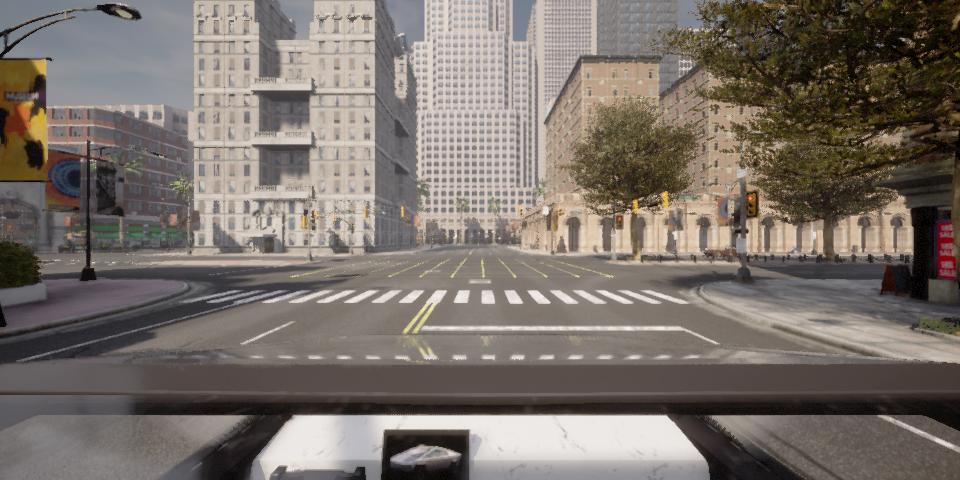
\includegraphics[width=0.8\textwidth]{parts/figuras/simulation-capture.png}
    \caption{A camera capture of the simulation. This camera was attached to the top of the car, and placed facing "front" relative to it.}
    \label{fig:simulation-screenshot}
\end{figure*}

Figure \ref{fig:simulation-screenshot} shows an example of a collected image from a vehicle camera in the simulation. Camera pose didn't reproduce its positioning in autonomous vehicles in the real world, as that is not relevant for measuring the system impact. An arbitrary positioning was used to help simulation monitoring, for example, to check if the vehicle was working as expected, didn't collide, among other problems that could happen during the experiment.

Table \ref{tab:my-table_1} presents memory and CPU consumption data for a single vehicle with 3 sensors that was created and integrated into the existing traffic manager of the simulation environment. In this simulated environment, the Elastic APM python agent creates several objects for monitoring and introspection, the memory spent is more than double the memory collected directly from the sensors.

\begin{table}[!htb]
\centering
\scalebox{0.83}{
\begin{tabular}{|l|l|l|l|}
\hline
    Usage                                       & Memory       & CPU  & Memory difference \\ \hline
without any data collection  & 29.0 MB & 0.44\% & - \\ \hline
with client data collection   & 38.9 MB & 0.55\% & 9.9 MB  \\ \hline
% 54.3 + 50.9 client + apm server memory values
% 0.57 + 0.1 client + apm server cpu values
with profiling data collection & 105.2 MB & 0.67\% & 76.2 MB  \\ \hline
\end{tabular}
}
\caption{Total memory and CPU comparison between collection methods. The simulation server is not accounted for.}
\label{tab:my-table_1}
\end{table}

Increase in CPU usage for the profiling solution was smaller than anticipated, our main hypothesis for this is that we are only monitoring a small number of objects (3 sensors) and the load is more memory and I/O based (for logging reasons). Total storage used after 1 hour of navigation was 441 MB, accounting for the images of the 2 cameras and 1 Lidar sensor.

New electric vehicles come equipped with an increasing number of cameras, the BYD Atto 3 has 5 cameras and the Tesla Model 3 currently has 9. To further evaluate the system load in respect to these kind of sensors only, we evaluated CPU and RAM usage against an increasing number of cameras. The cameras used a default setup of 960x480 resolution and 120 degrees field of view. Results are presented in Table \ref{tab:my-table_3}.

\begin{table}[!ht]
\centering
\scalebox{0.83}{
\begin{tabular}{|l|l|l|l|}
\hline
\# of cameras      & Memory       & CPU  \\ \hline
1  & 34.1 MB & 0.57\%  \\ \hline
2  & 38.4 MB & 0.82\%   \\ \hline
3  & 41.5 MB & 1.04\%  \\ \hline
4  & 44.3 MB & 1.19\%   \\ \hline
5  & 46.4 MB & 1.42\%  \\ \hline
6  & 48.0 MB & 1.58\%   \\ \hline
7  & 49.4 MB & 1.76\%  \\ \hline
8  & 51.2 MB & 1.95\%  \\ \hline
9  & 52.7 MB & 2.13\%  \\ \hline
\end{tabular}
}
\caption{Total memory and CPU usage for an increasing number of cameras, both increase linearly with the number of cameras.}
\label{tab:my-table_3}
\end{table}

To experiment with SOTA self driving models, Table \ref{tab:table2} presents impact on memory and CPU from collecting data for a Transfuser \cite{chitta2022transfuser} agent, the winner of one of the CARLA Challenges event. Sensor setup was reproduced from the authors github repository\footnote[9]{https://github.com/autonomousvision/transfuser/} containing 3 cameras (with higher resolution than previous baseline experiment), one lidar sensor, an IMU, a GNSS and a speedometer. A total of 7 sensors. As reference, for the Transfuser model training, each camera has, in addition to RGB, depth maps and semantic segmentation data.

\begin{table}[!ht]
\centering
\scalebox{0.83}{
\begin{tabular}{|l|l|l|l|}
\hline
    Usage                                       & Memory       & CPU  & Memory difference \\ \hline
without extra collection  & 29.4 MB & 0.4\% & -  \\ \hline
with sensor data collection   & 45.8 MB & 0.91\% & 16.4 MB  \\ \hline
% 58.8 + 50.4 (client + apm server memory values)
% 1.07 + 0.2 (client + apm server cpu values)
with profiling data collection & 109.2 MB & 1.09\% & 79.8 MB   \\ \hline
\end{tabular}
}
\caption{Total memory and CPU comparison between data collection methods for the Transfuser agent. Total sensor count in the CARLA simulator: 7. Simulation server is not accounted for in used memory.}
\label{tab:table2}
\end{table}

The same baseline model was used for navigation (not the Transfuser model), so the usage without the data collection in practice is the same. We can observe that the memory spent in the sensor data collection method increased around 20\%, this can be attributed to the growth of sensors on the vehicle. On the other hand, the memory from the APM data collection tools kept being much more significant, even though it didn't scale with the number of sensors like it did in the first experiment. For this experiment, the total storage used after 1 hour of data collection was 3.1 GB, This big increase in used memory is attributed to the increase in amount of sensors, number of cameras and camera resolution. Lidar setup didn't change between experiments.

To better understand the impact this system would have on a vehicle in the real world, we considered the Delphi Audi zFAS, which is a central driver assistance controller released in 2018, for Audi's A8 model. The controller owns a 4 GB SDRAM, DDR3L-1866, so with the transfuser setup (7 sensors) that translates to 1.1\% of total memory usage with the direct sensor collection, and 2.6\% with the APM data collection, a neglectable impact on a 6 year old controller. Additionally, the camera test still shows a feasible expenditure with 9 cameras: 52.7MB or 1.32\% of the total controller memory.

Autonomous vehicles have security and decision modules that need to access data with minimum latency. For this reason, CPU and memory assets must be rationalized as much as possible, the presented sensor data collection mechanism is able to meet that necessity.

In a nutshell, the costlier performance of the APM solution was expected due to the software evaluation infrastructure built around it. In physical vehicles, on the other hand, the extra load will be less than that presented in this work, considering that instead of a python profiler, a profiler is used at the vehicle operational system level.

The increase in amount of storage needed for the extra module is relevant as we show that for the transfuser model, this would be around 3GB for 1 hour. Camera and lidar data are raw and represent the biggest part of this volume, with 2.8GB dedicated to the 960x480 resolution images from the 3 cameras.

\section{A traffic monitoring experiment}

Considering that starting code is available for data collection, an additional data collection experiment was designed to take advantage of it.

In order to evaluate a simple traffic monitoring application, three "monitor vehicles" were placed in the simulation. For each vehicle, GNSS and speedometer sensor data was collected in the same way it was done in the previous experiment.

At the CARLA simulation, a map called Town10HD\_Opt was selected\footnote{https://carla.readthedocs.io/en/latest/map\_town10/}. This map's road network consists of a grid layout, including numerous different junctions and traffic lights.

A light and a heavy traffic scenario were considered, one with only the three vehicles in the simulation, allowing for top speed in the selected map, and one with the monitor vehicles and another 100 cars, to examine the heavy traffic scenario.

\begin{figure*} [!ht]
    \centering
    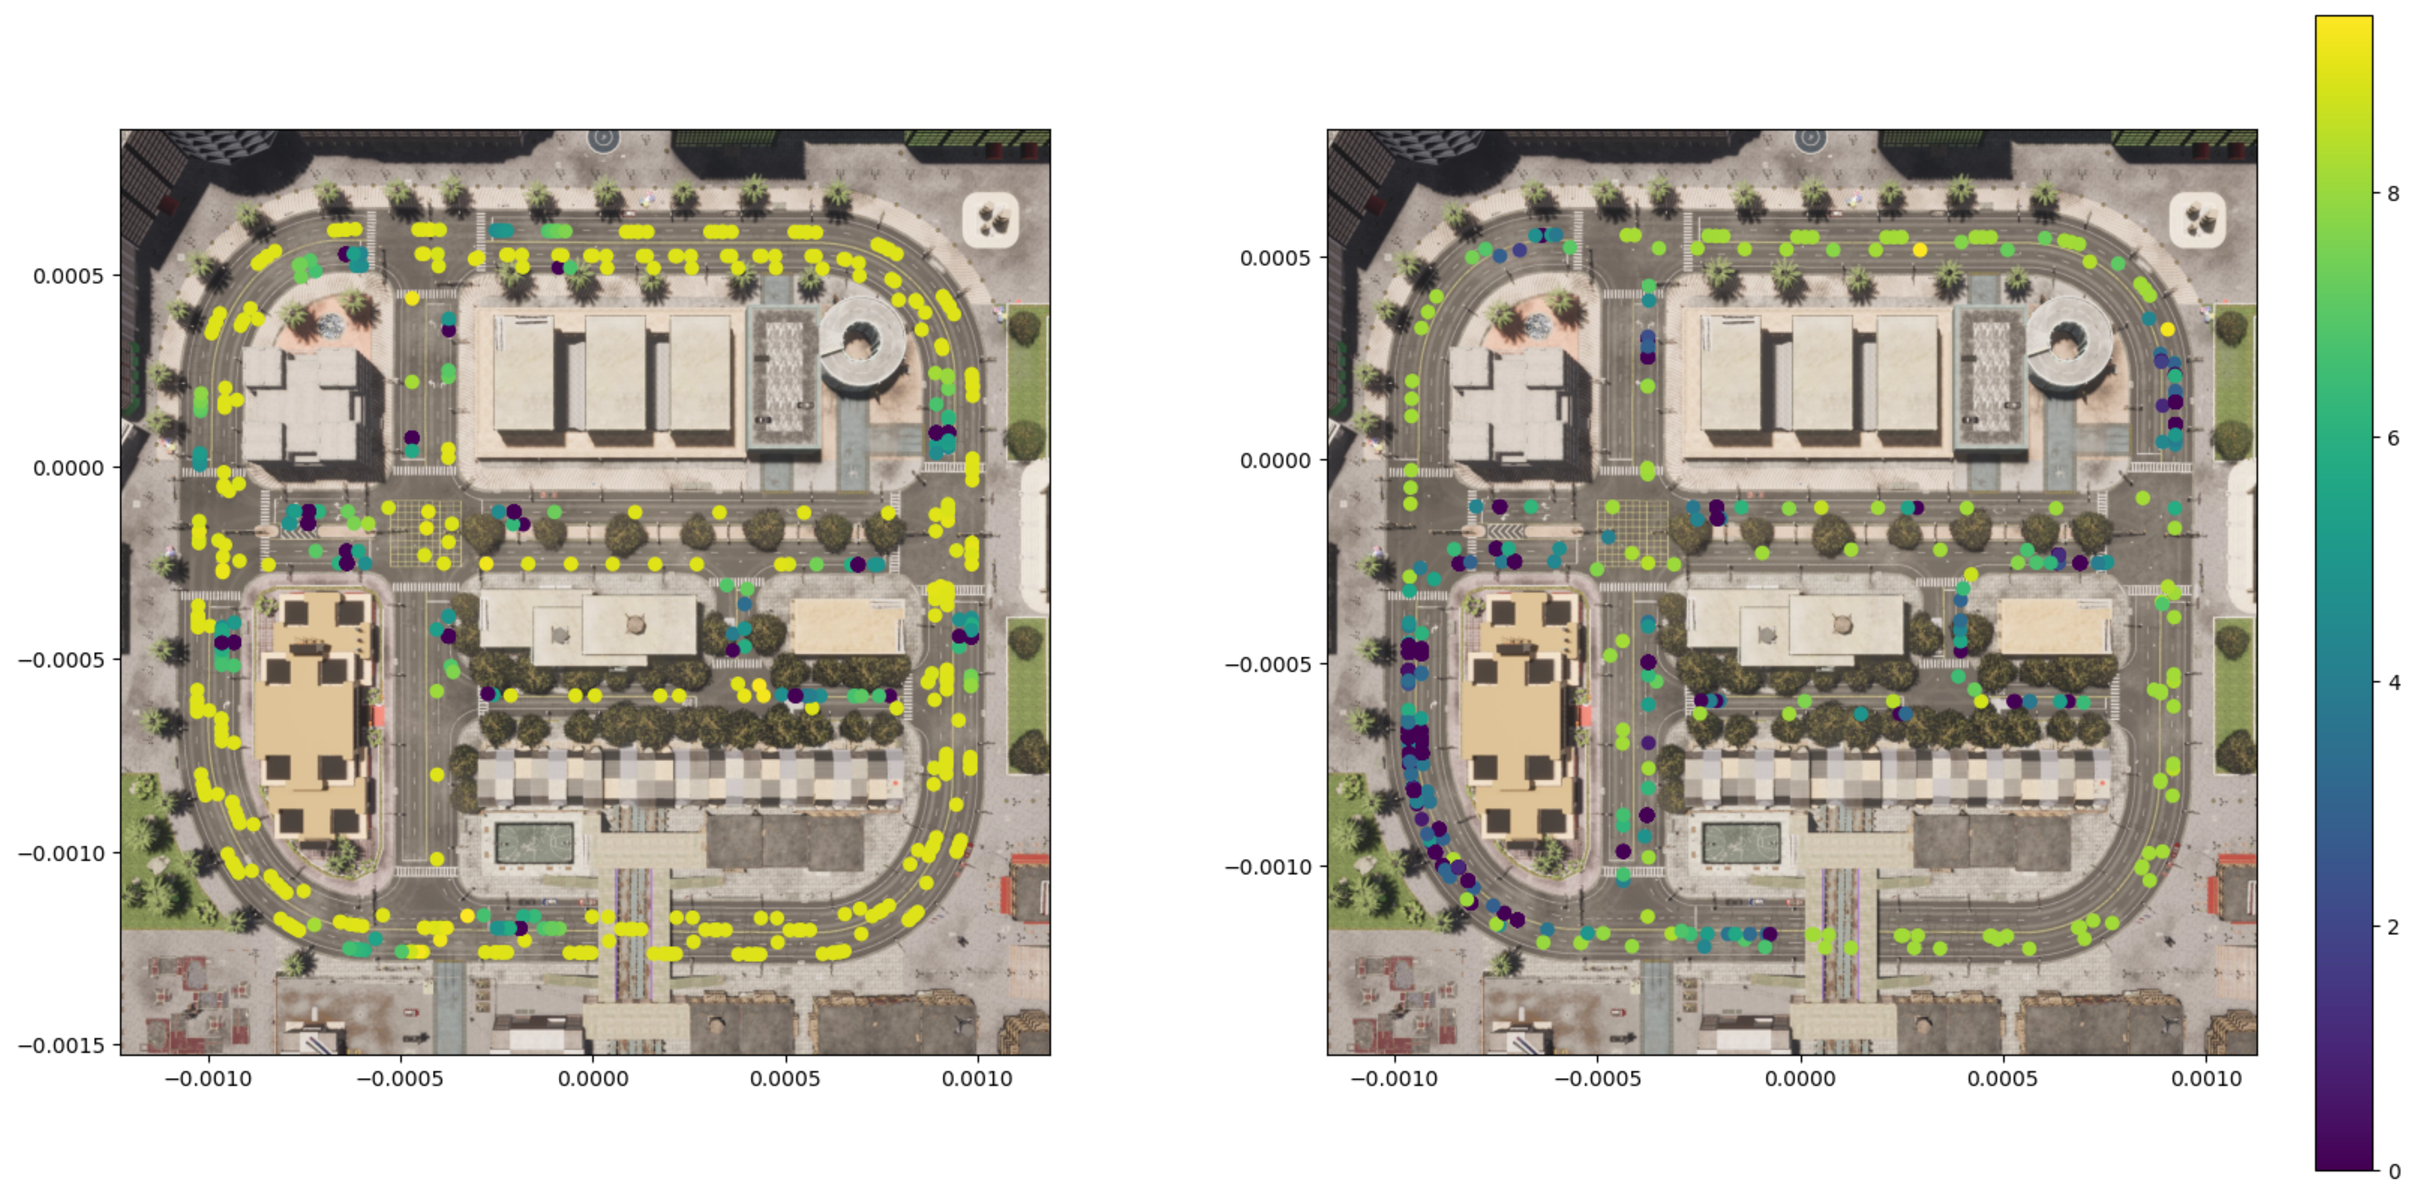
\includegraphics[width=0.9\textwidth]{parts/figuras/traffic-comparison.pdf}
    \caption{Traffic comparison, on the left the light traffic simulation, and on the right the heavy one. Points represent the vehicle location and the speed during collection step. Right color map is represented in meters per second.}
    \label{fig:traffic-monitoring}
\end{figure*}

Each vehicle built a log of the collected data, the log was monitored in real time and data was collected for 20 minutes. At the end of the simulation, map data was fused with the GNSS and speed data from the vehicles to generate the proposed traffic monitor.

Figure \ref{fig:traffic-monitoring} depicts the experiment end result. Its possible to observe that even in the light traffic scenarios, some points of the road have a lower mean speed. This points are present in junctions or traffic lights.

Another thing that was expected was the low average speed even for the light traffic scenario (~8.5 m/s or 30.6 km/h). This happened because the selected map represent a "downtown" location, consisting of several junctions and traffic lights, that would naturally lower the speed of passing vehicles.

As expected, in the heavy scenario situation, traffic light and junctions are the places with the biggest impact, its possible to observe a large traffic jam on the lower left corner of the map. Considering the simplicity of the generated code, it can be reused to evaluate light and heavy in all other CARLA maps.

If a minimal number of vehicles share this kind of data with a single, centralized server, its possible to have real time speed data with a reasonable error. The error rate increases with the decreasing of number of vehicles, as data gets "old" until another vehicle passes by the location to metrify speed again.

\section{Data transmission simulation}

In order to create the network experiments part of the cooperative perception simulation, we built a new application for communication simulation on top of previous experiments code. These new experiments do not use APM methods for data collection, and rely solely on CARLA`s sensor data implementation.

The new addition takes advantage of the Carlanet project \cite{cislaghi2023simulation}, in which Omnet and CARLA communication is implemented as a message queue with ZeroMQ.

\begin{figure*} [!ht]
    \centering
    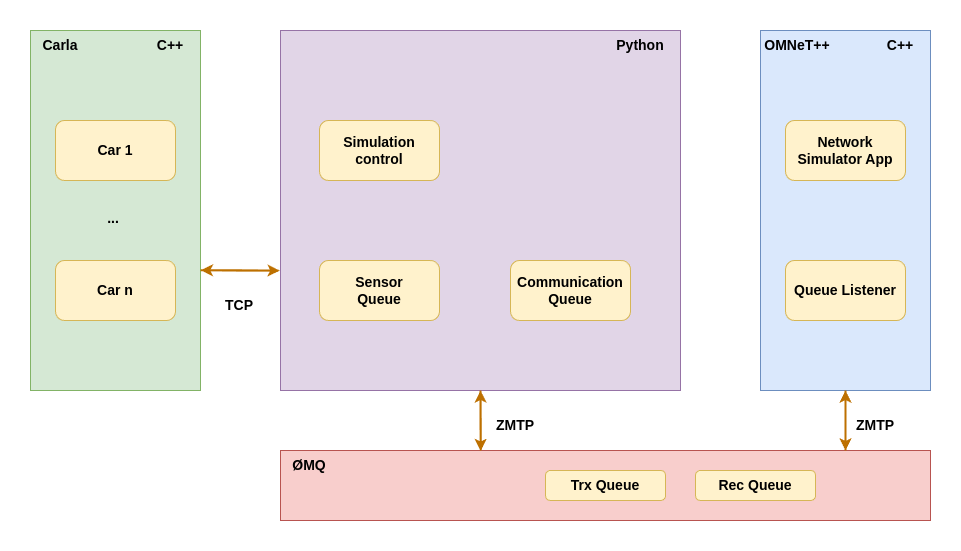
\includegraphics[width=0.9\textwidth]{parts/figuras/implementation-dissertacao.drawio.png}
    \caption{Block diagram containing the simulation framework components. Carla and experiment communicate via TCP and Omnet++ communication happens through ZeroMQ.}
    \label{fig:block-diagram}
\end{figure*}

As a significant amount of stack has been added to the experiment code, Figure \ref{fig:block-diagram} portraits the new overall setup. Communication with CARLA maintains the TCP standard with ports 2000, 2001 and 2002. When sensor data is available for transmission, or when the vehicle controller is asked for, sensor data is sent to OMNET++ through a transmission queue for network simulation. 

Default format for data transmission in the Carlanet setup is json messages, so when camera image data is transmitted, it has to be base64 encoded and then decoded as utf-8 to text, as bytes are not serializable in json format. An example of the json message is presented below in "Code" \ref{json:example}.

\begin{lstlisting}[caption={json message example},label={json:example}]
{
   "message_type":"GENERIC_RESPONSE",
   "simulation_status":0,
   "user_defined":{
      "msg_type":"VEHICLE_DATA",
      "camera_data":"gHx8/4F9ff+BfX3/gX19/.../gX19/",
      "actor_positions":[
          {
             "actor_id":"carlaNodeCar_1",
             "position":[
                325.1853942871094,
                1.9907456636428833,
                0.0019066429231315851
             ],
             "rotation":[
                -0.010655094869434834,
                0.06594514101743698,
                -0.00012207029067212716
             ],
             "velocity":[
                6.835569858551025,
                0.008157790638506413,
                8.010864007701457e-07
             ],
             "is_net_active":true
          }
      ]
   }
}
\end{lstlisting}

To keep both simulations synchronized, a "Simulation step" message is also exchanged between the simulations. At every simulation step, vehicle location and speed are sent to Omnet++. This is needed to correctly execute the 5G network simulations.

With the initial communication setup done, we reproduce the traffic monitoring experiment with location and speed data being transmitted from the vehicles to a 5G antenna placed in the center of CARLA`s TOWN01, the smallest map available.

The antenna is connected to a Remote Service Agent that sits in the python part of the code. When a new data message arrives, it performs network simulation (from car to antenna) at Omnet++ and forwards it to the experiment Receiving Queue for the Remote Agent to process. Once in the Receiving Queue, the remote service 
saves it to the local file system for processing by reusing code from the traffic monitoring experiment.

The following Sequence Diagram in Figure \ref{fig:sequence-diagram} represents how the experiments were performed. An initial configuration phase is done where all the simulators are started and configured. Omnet++ contains the trigger to start the entire experiment, after started, it triggers the experiment configuration both in itself and in carla, where the configured Actors are placed and vehicle control is configured.

\begin{figure*} [h!]
    \centering
    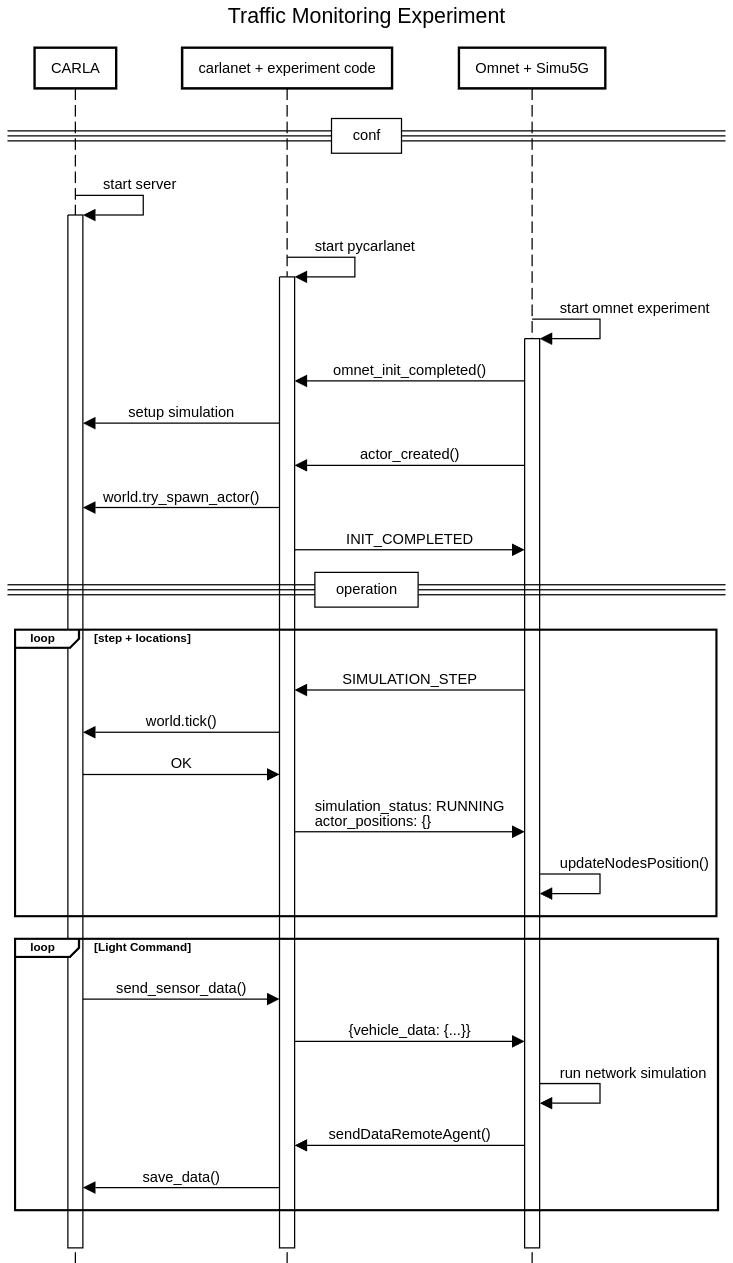
\includegraphics[width=0.5\textwidth]{parts/figuras/traffic monitoring sequence diagram.png}
    \caption{Sequence diagram representing the data flow in the experiment application. After an initial configuration stage, 2 communication loops are executed: One for simulation synchronization and other for data sharing.}
    \label{fig:sequence-diagram}
\end{figure*}

Two communication loops are then initiated, the "Simulation step" and the "Vehicle data" messages start being exchanged by using the ZeroMQ Service.

Traffic monitoring experiment is run for TOWN01, with a remote data service to represent an ITS traffic management system, again with 0 and 100 cars.

Results show the same standard as previous traffic monitoring experiment: average speed around traffic lights drop significantly when the map is full of cars. 

Results can be seen at Figure \ref{fig:traffic-monitoring-network}. datapoints are sparser even though the same number of monitor cars were used, that is due to the fact that the collection average time for each location and speed was increased from 3 to 9 seconds, in adaptations from the initial code to the Carlanet standard.

\begin{figure*} [!ht]
    \centering
    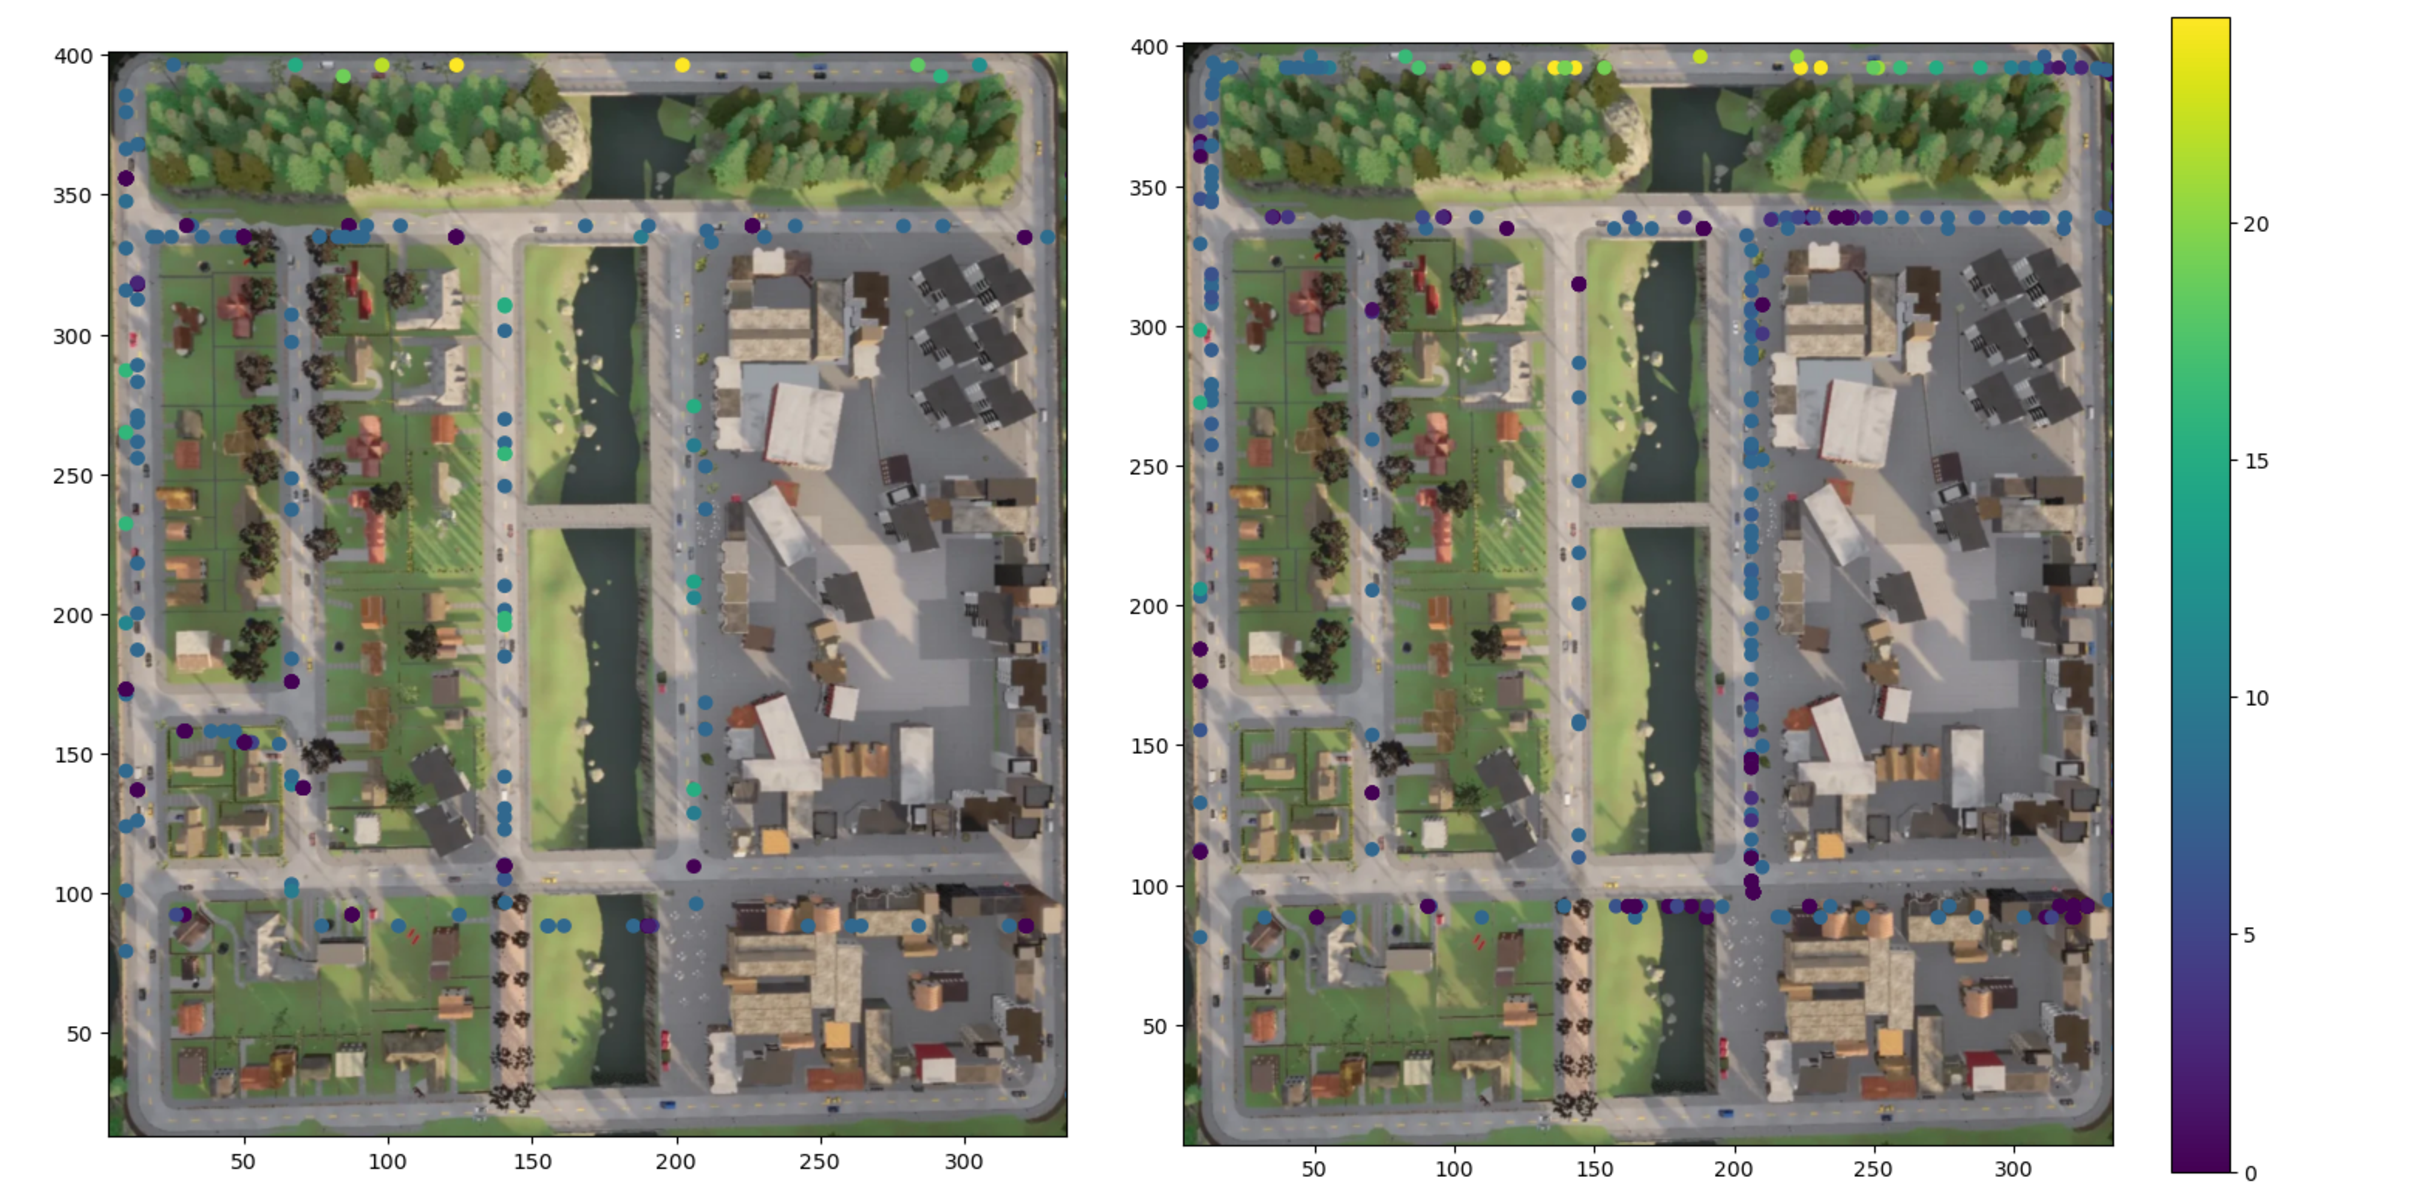
\includegraphics[width=0.9\textwidth]{parts/figuras/traffic-comparison-network.pdf}
    \caption{Traffic comparison, on the left the light traffic simulation, and on the right the heavy one. Points represent the vehicle location and the speed during collection step. Right color map is represented in meters per second.}
    \label{fig:traffic-monitoring-network}
\end{figure*}

Average speed was 18 km/h at the "No traffic" simulation and 10.8 km/h at the "High traffic" one. A thing to note is that Town01 is actually bigger than Town10, so an addition of 100 cars didn't have the same impact as it had in the previous traffic monitoring simulation.

\begin{figure*} [h!]
    \centering
    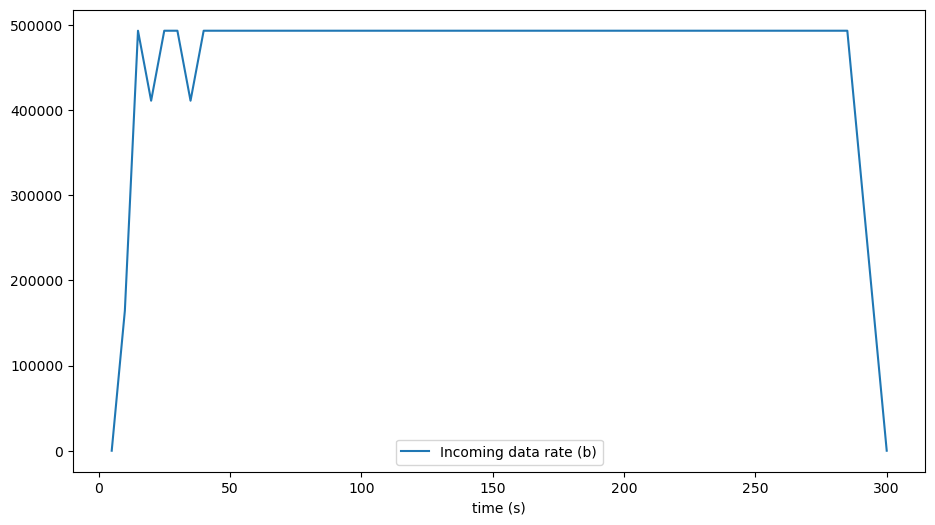
\includegraphics[width=0.7\textwidth]{parts/figuras/bitrate-1-car.png}
    \caption{Bit rate of a single vehicle during simulation time. Two messages are exchanged, Simulation step and traffic monitoring.}
    \label{fig:bitrate-1-vehicle}
\end{figure*}

In an additional experiment made to measure channel usage, figure \ref{fig:bitrate-1-vehicle} shows the Bit rate of the data transmissions from a single car for around 6 minutes of simulation: A total of 61,68 KB/s considering both Simulation step and traffic monitoring messages.

Our hypothesis for the first fall in the Bit rate after an established connection is occlusion or some sort of signal interference that was not purposely added to the simulation.

Considering that a 5G antenna capacity is 10 Gbps, both messages account for 0.049\% the maximum channel usage. If a dedicated antenna is considered, a single one is capable of receiving messages from 2040 vehicles at the same time.

Current B5G/6G research estimate big improvements with bitrates getting up to 100 Gbps, further increasing the feasibility of a virtual data infrastructure for traffic monitoring purposes.

\section{Cooperative Perception simulation framework for V2X Security experiments}

Building upon our previous data collection and transmission experiments, we developed a integration framework between CARLA and Simu5G simulators to enable cooperative perception testing focused on V2X cybersecurity. This integration addresses the critical need for realistic simulation environments that can model both complex traffic scenarios and 5G network communications simultaneously, particularly when evaluating security aspects like jamming and spoofing attacks.

The integration architecture, called B5GCyberTestV2X\_CARLANet, is the central connection point between CARLA and Simu5G. This framework enables vehicles within the CARLA environment to share sensor data through simulated 5G connections, creating a bootstrapped environment for cooperative perception algorithms under various security threat scenarios.

Within B5GCyberTestV2X\_CARLANet, several key submodules work together to facilitate the operation and programming of use case scenarios. Figure \ref{fig:B5GCyberTestV2X} shows the system architecture. The "Data" submodule collects information from sensors incorporated into the CARLA simulator, sending this information simultaneously to the TX submodule and the "Fusion" submodule. Meanwhile, the "Control" submodule manages vehicle actuators within the CARLA environment, ensuring precise control over vehicle behavior based on cooperative perception inputs. Any algorithm can be used with the control submodule, including CARLA's auto pilot feature. This setup creates a closed feedback loop where vehicles can share sensor data, process information from other vehicles, and adjust their behaviors accordingly.

\begin{figure*} [!ht]
    \centering
    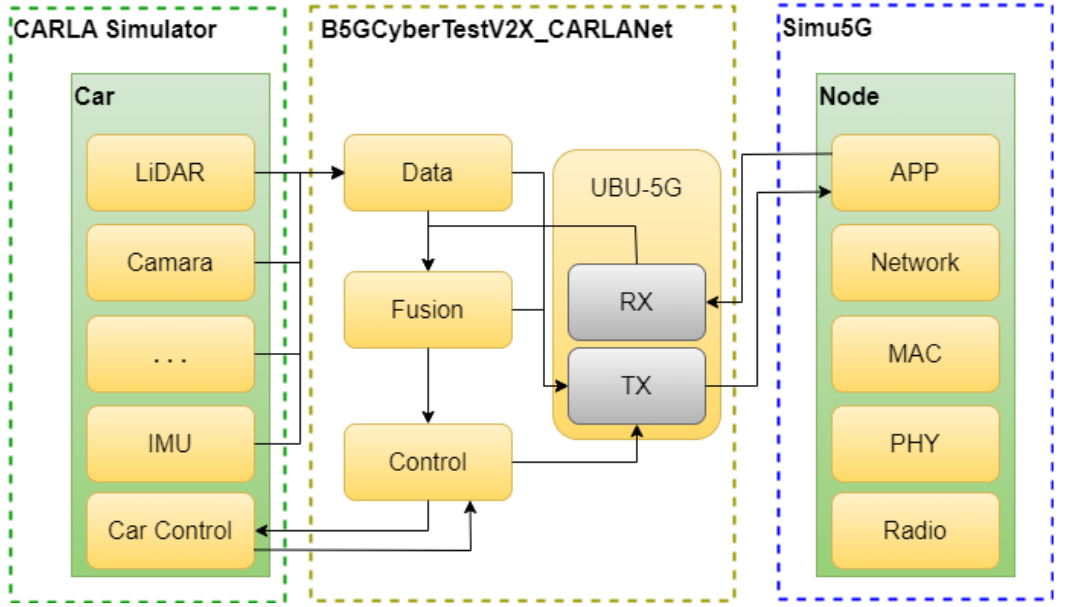
\includegraphics[width=0.85\textwidth]{parts/figuras/B5GCyberTestV2X_CARLANet.png}
    \caption{Block diagram depicting the B5GCyberTestV2X\_CARLANet architecture for integration between CARLA and Simu5G simulators. The diagram illustrates the data flow from vehicle sensors (LiDAR, Camera, IMU) through the central integration module to the Simu5G network simulation. Key components include the Data submodule for sensor acquisition, Fusion for data integration, Control for vehicle actuation, and the UBU-5G module containing RX/TX components that facilitate bidirectional communication with the Simu5G network stack.}
    \label{fig:B5GCyberTestV2X}
\end{figure*}

The communication between CARLA and B5GCyberTestV2X\_CARLANet continues to utilize TCP with Protocol Buffers (protobuf) for efficient data serialization, operating across ports 2000, 2001, and 2002. For the connection between B5GCyberTestV2X\_CARLANet and Simu5G, we continue to use the ZeroMQ service with the ZMTP protocol, working on top of the Carlanet project.

Our simulation workflow begins with the B5GCyberTestV2X\_CARLANet module initializing both simulators using configurations present in a single configuration file. During operation, an iterative cycle processes sensor data collection from CARLA vehicles, transmission of this data through the simulated 5G network, reception by other vehicles, fusion with local sensor data, and control actions based on the combined information. 

For the cooperative perception tests, Figure \ref{fig:B5GCyberTestV2X-use-case} depicts a use case that was implemented involving two autonomous vehicles communicating via V2V connections. In this scenario, Car 1 collects sensor data and transmits it to Car 2 through the simulated 5G network. Car 2 then fuses this data with its own sensor readings and executes control algorithms based on this combined information. 

\begin{figure*} [!ht]
    \centering
    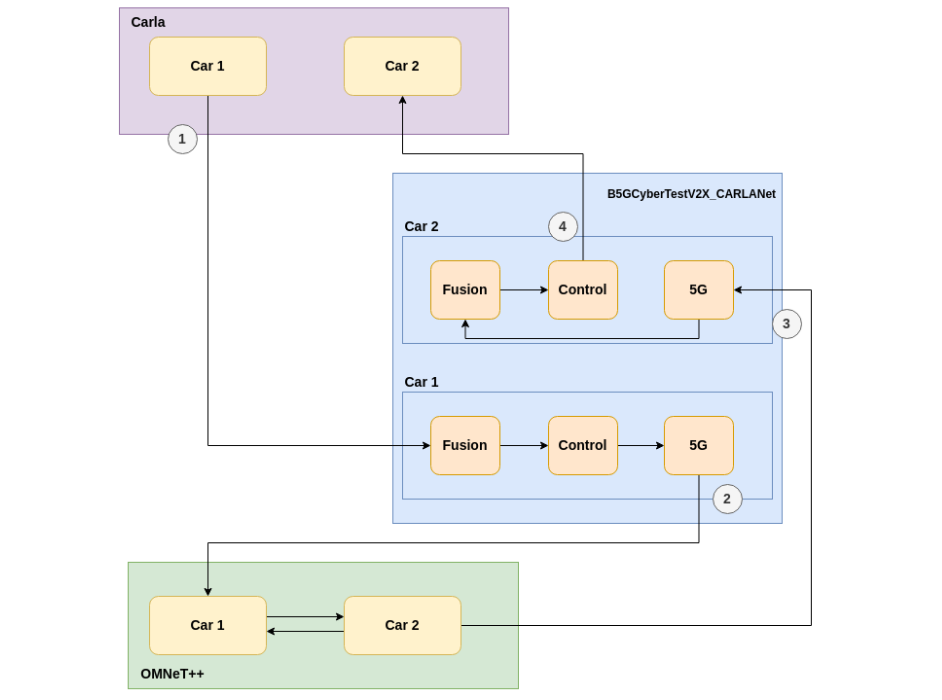
\includegraphics[width=0.95\textwidth]{parts/figuras/B5GCyberTestV2X_use_case.png}
    \caption{Block diagram of a shared perception use case in the B5GCyberTestV2X framework. 1. Car 1 in CARLA sends sensor data to the B5GCyberTestV2X\_CARLANet module; 2. data is transmitted to the OMNeT++ environment for network simulation; 3. Car 2 receives the processed data through its 5G module; 4. fusion and control components process the combined information to execute appropriate actions in the CARLA simulator.}
    \label{fig:B5GCyberTestV2X-use-case}
\end{figure*}

For monitoring and logging, each component of the system features its own implementation managed by the experiment code. Additionally, we used CARLA's Recorder feature to document events during simulation, allowing for detailed post-analysis and reproducibility of results. 

This integration framework represented a significant advancement in simulation for autonomous vehicle research in the cybersecurity domain. By combining traffic simulation with realistic 5G network modeling, the framework enables the testing of cooperative perception systems under various security scenarios.

\section{A Simulation Dataset for Vehicular Cybersecurity experiments}

Building on top of the developed data sharing framework, a series of standalone experiments were conducted to research vehicular cybersecurity, specifically focusing on Vehicle-to-Everything (V2X) communication security and spoofing attack detection.

This research addressed critical vulnerabilities in V2X systems where malicious actors can inject false information, disrupting traffic flow and compromising autonomous vehicle safety. The study combined hardware-level signal analysis (Direction of Arrival) with AI vision detection methods (YOLO V8) to develop a new method for detecting spoofing attacks and identifying the physical location of malicious senders.

\begin{figure*} [!ht]
    \centering
    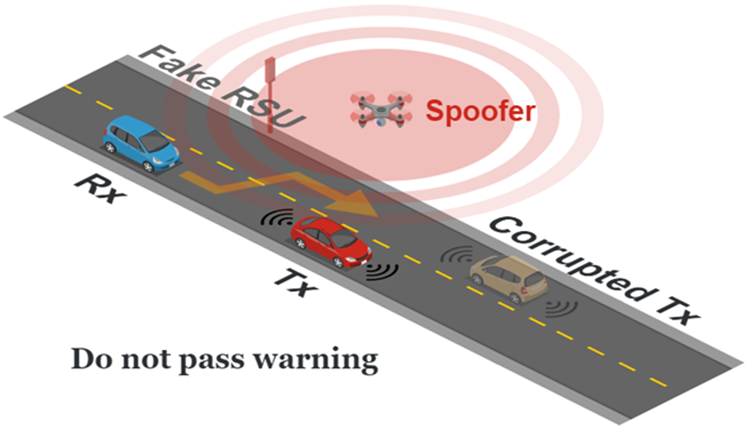
\includegraphics[width=0.5\textwidth]{parts/figuras/DoNotPassWarning.png}
    \caption{Do Not Pass Warning illustration depicting a drone-based attack where a malicious actor deploys a counterfeit roadside unit (RSU) to inject corrupted data into the vehicle network. The compromised signals disrupt V2X communications between the transmitting and receiving vehicles, creating unsafe conditions during passing maneuvers.}
    \label{fig:do-not-pass-warning}
\end{figure*}

Three autonomous driving scenarios were simulated using the CARLA simulator to generate the datasets. The first scenario, depicted in Figure \ref{fig:do-not-pass-warning}, "Do Not Pass Warning", represents a common highway situation where vehicles need to make overtaking decisions. This scenario involves communication between vehicles to ensure safe passing maneuvers, particularly critical when one vehicle needs to determine if there is sufficient time and space to overtake another vehicle safely.

The second scenario, "Vulnerable Road User Alerts at Blind Intersections", is illustrated in figure \ref{fig:vulnerable-road-user} addresses the challenge of detecting and responding to pedestrians at intersections with limited visibility. This scenario is particularly relevant it is a common occurrence in urban environments where buildings or other obstacles can obstruct a vehicle's direct line of sight.

\begin{figure*} [!ht]
    \centering
    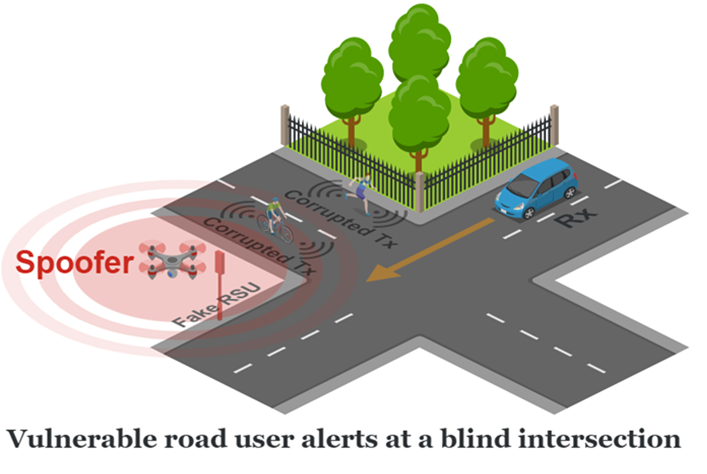
\includegraphics[width=0.5\textwidth]{parts/figuras/VulnerableRoadUserAlerts.png}
    \caption{Vulnerable Road User Alert system being compromised at a blind intersection. A drone-based attack using fake infrastructure signals disrupts critical safety communications between vehicles and pedestrians, creating heightened risk at an already visibility-limited crossing.}
    \label{fig:vulnerable-road-user}
\end{figure*}

The third scenario is called "Left Turn Assist" (available in figure \ref{fig:left-turn-assist}) focuses on the complex decision-making process required when vehicles execute left turns at intersections, requiring coordination and communication between multiple vehicles to prevent collisions.

\begin{figure*} [!ht]
    \centering
    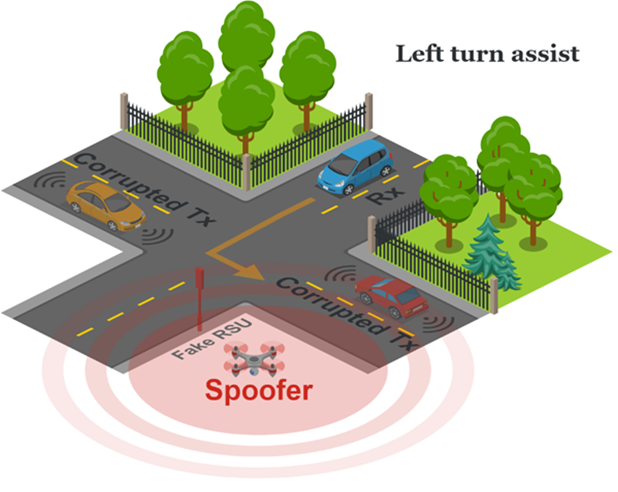
\includegraphics[width=0.5\textwidth]{parts/figuras/LeftTurnAssist.png}
    \caption{Left Turn Assist system compromised by a drone attack that uses counterfeit infrastructure signals to interfere with vehicle communications at the intersection. The spoofed data affects vehicles' ability to safely coordinate left turns, creating potential collision risks.}
    \label{fig:left-turn-assist}
\end{figure*}

For each of these scenarios, we collected two distinct subsets of data. The first subset captured normal operation data, where V2X communications functioned as intended, resulting in safe navigation and accident prevention. The second subset contained attack scenario data, where communications were compromised through spoofing attacks, leading to potential or actual accidents.

The dataset includes temporal sets of: vehicle position coordinates in three dimensions, vehicle orientation including pitch, yaw, and roll measurements, vehicle velocity vectors, camera captures from vehicle-mounted sensors, pedestrian position data where applicable, drone position and orientation data, and timestamp information for synchronization purposes.

In the Do Not Pass Warning scenario, data was collected from three vehicles and one drone. The normal operation subset demonstrated successful overtaking maneuvers where vehicles maintained safe distances based on accurate position and velocity information. The attack scenario subset revealed how spoofed location data led to unsafe passing decisions, resulting in collisions.

Figure \ref{fig:vulnerable-road-user-attack} shows the Vulnerable Road User scenario. In this scenario, we gathered data from two vehicles, one pedestrian, and one drone (the cyclist was considered a vehicle to the simulation). Normal operation data showed the system successfully detecting and responding to pedestrians at blind intersections. The attack scenario data documented instances where compromised sensor information resulted in vehicles failing to detect or appropriately respond to pedestrian presence.

\begin{figure*} [!ht]
    \centering
    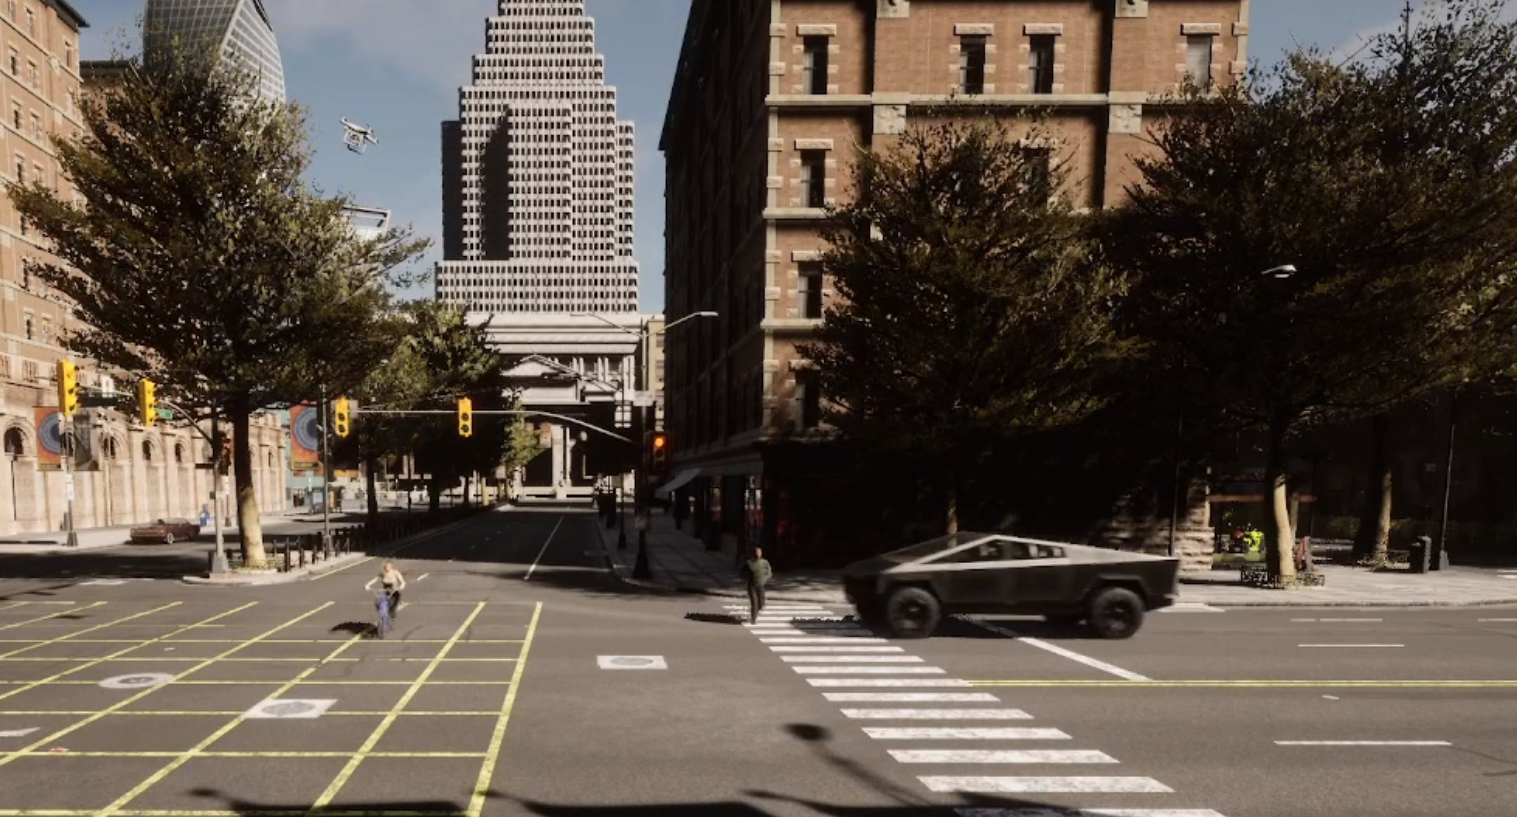
\includegraphics[width=0.8\textwidth]{parts/figuras/vulnerable-road-user.png}
    \caption{Simulation scenario of Vulnerable Road user use case, the vehicle can be seen about to collide with the pedestrian. The Spoofer drone can be seen in the sky, at the upper left corner of the image.}
    \label{fig:vulnerable-road-user-attack}
\end{figure*}

For the Left Turn Assist scenario, three vehicles and one drone were monitored. The normal operation subset captured successful left turn maneuvers enabled by proper V2V communication. The attack scenario subset illustrated how manipulated position and velocity data could lead to incorrect turn timing decisions and potential accidents. An example of attack situation can be seen in figure \ref{fig:left-turn-assist-attack}.

\begin{figure*} [!ht]
    \centering
    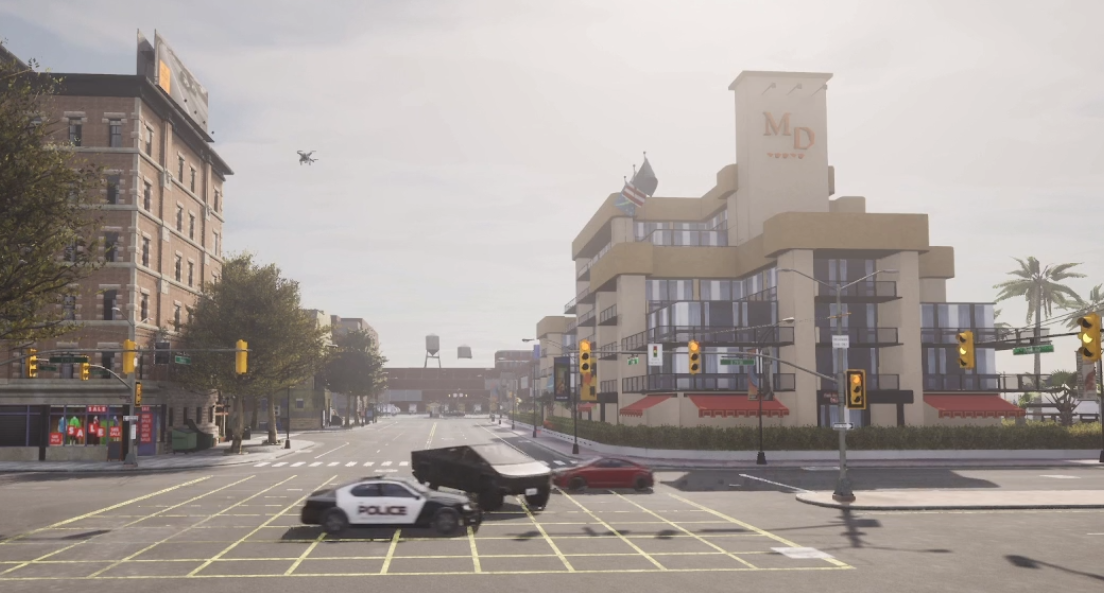
\includegraphics[width=0.8\textwidth]{parts/figuras/left-turn-assist-attack.png}
    \caption{A picture illustrating an attack in the Left Turn Assist scenario. The Tesla Cybertruck does a improperly timed left turn and ends up colliding with a police vehicle. The spoofer drone can be seen in the sky, close to the intersection.}
    \label{fig:left-turn-assist-attack}
\end{figure*}

The spatial and temporal data collected enabled accurate identification of malicious transmitters' physical locations through Direction of Arrival (DoA) estimation techniques. Furthermore, having both normal operations and attack scenarios helped training and validating our AI-based framework for attacker classification and countermeasure selection.

\section{Generating data for vision model finetuning}

To enable robust drone detection capabilities for identifying potential attackers, a specialized dataset was created for fine-tuning the YOLOv8 object detection model. The complete dataset comprises 4,824 annotated images focused on drone detection across various environments and conditions. This dataset was divided into a training set containing 3,877 images (80\% of the total) and a validation set of 947 images (20\% of the total).

A significant portion of the dataset was generated using the CARLA simulation environment. The data collection process involved placing stationary drones at strategic locations across different CARLA maps. Due to limitations in the simulation software's drone physics capabilities at the time of data collection, the drones remained in fixed positions throughout the collection process. Given the technical constraints of implementing new vehicle models in CARLA, a single drone model was utilized, the model and its dimensions inside the simulation are available in Figure \ref{fig:drone-dimensions}, though its appearance was varied through random color alterations to introduce visual diversity.

\begin{figure*} [!ht]
    \centering
    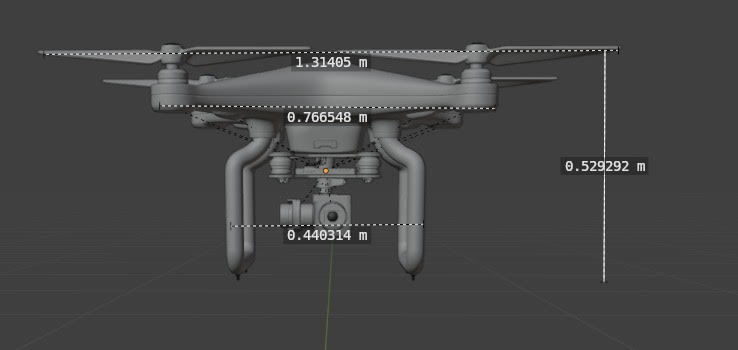
\includegraphics[width=0.8\textwidth]{parts/figuras/drone-dimensions.jpg}
    \caption{A picture of the drone model inserted in the simulation}
    \label{fig:drone-dimensions}
\end{figure*}

The image collection process in the simulation environment was conducted through automated vehicle routes with mounted cameras. These vehicles would navigate through the city environments, capturing images at approximately 0.3-second intervals. Each collection session lasted several minutes, during which simulation parameters were periodically randomized to create diverse scenarios. These parameters included weather conditions and time of day, ensuring the dataset captured a wide range of lighting conditions and atmospheric effects. One example can be seen in Figure \ref{fig:drone-simulation-capture}.

\begin{figure*} [!ht]
    \centering
    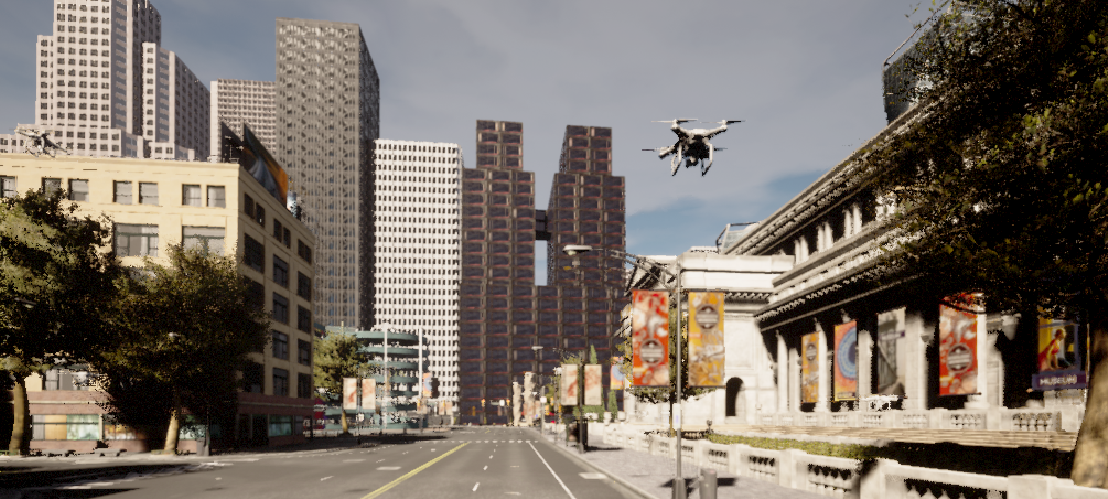
\includegraphics[width=0.8\textwidth]{parts/figuras/drone-simulation-capture.png}
    \caption{One of the raw images generated by the simulation for further annotation. A drone can be seen on the right with the sky as the background, while a second drone is a little harder to see is at the far left, with some buildings in the background.}
    \label{fig:drone-simulation-capture}
\end{figure*}

To supplement the simulated data and enhance the model's generalization capabilities, synthesized images showing drones in various lighting conditions and backgrounds were also incorporated in the dataset, as well as augmented versions of base images.

The annotation process required careful attention to detail and consistency. Each image received manual bounding box annotations indicating drone locations within the frame. A single-class labeling approach was maintained, focusing solely on drone detection, as this aligned with the specific need to identify potential attack sources. Annotation standards remained consistent across the entire dataset to ensure data quality.

The YOLOv8 model was trained with specific parameters optimized for this use case. The input format followed the NCHW standard (Batch, Channels, Height, Width) with image dimensions of 3×640×640 pixels. A batch size of 32 was used with the Adam optimizer and Cosine Annealing for learning rate scheduling. The initial learning rate was set to 0.005, gradually decreasing to 1.0e-05 throughout the training process. The model trained for 200 epochs to ensure proper convergence.

The performance metrics from the training process demonstrated strong detection capabilities. The model achieved a Mean Average Precision (mAP50) of approximately 0.9, indicating excellent accuracy in drone detection at the standard 50\% Intersection over Union (IoU) threshold. The more stringent mAP50-95 metric reached approximately 0.6, showing robust performance across varying IoU thresholds. Both precision and recall metrics stabilized near 0.9, indicating balanced performance in terms of false positives and false negatives.

The fine-tuned model became an important component of the larger spoofer detection framework. The high-accuracy drone detection capabilities were essential for identifying potential attack sources in V2X environments, complementing the signal processing approaches with visual confirmation of threat vectors. The model's reliable performance across various conditions enhanced the framework's overall ability to detect and respond to spoofing attacks in most real-world scenarios (at low lighting the results were not as good).

\section{Future Works: Security Challenges and Opportunities in V2X Cooperative Perception}

While significant progress has been made in establishing the B5GCyberTestV2X framework, training detection models, and simulating attack scenarios, several promising research directions remain unexplored. Building on our current foundation, several advanced research areas can be considered.

In the area of attack detection and mitigation, more sophisticated anomaly detection algorithms could be developed to identify vehicles purposely sharing incorrect location and speed data. This might include implementing real-time trust scoring mechanisms for data sources based on consistency and behavioral patterns. Additionally, adaptive countermeasures could be designed to automatically respond to different types of V2X attacks beyond the drone-based spoofing scenarios already simulated.

For resilient cooperative perception, future work could investigate predictive algorithms that maintain accurate environmental awareness during communication disruptions or jamming attacks. A critical challenge to address would be developing conflict resolution strategies when vehicle sensors and cooperative perception data provide contradictory information, such as when an object is placed in front of a vehicle in map data but not detected by onboard sensors.

Simulation capabilities could be further expanded to better model real-world scenarios. Additional network simulation tools might be integrated to model more complex attack vectors. The implementation of moving drone models with realistic physics would enhance the fidelity of aerial attack simulations. Furthermore, scenarios could be developed for testing system resilience against coordinated multi-vector attacks involving multiple malicious actors, providing insights into system vulnerabilities.

Looking to real-world applications, hardware-in-the-loop testing using the simulation framework connected to actual vehicle systems could be designed. Methodologies for transferring security insights from simulation to real-world V2X systems would be essential for practical implementation.

By exploring these research directions, the security and reliability of cooperative perception systems in autonomous driving could be further improved, making them more resilient against sophisticated cyber attacks and ensuring their robust operation in diverse real-world scenarios.